\documentclass[presentation]{subfiles}

\onlyinsubfile{
  % \usepackage[citestyle=numeric,backend=bibtex]{biblatex}
  % \bibliography{~/Library/texmf/bibtex/bib/local/references}
  % \beamertemplategridbackground[1mm]
}


\begin{document}
% \section*{Introduction}

% \frame<1-3>[frame1]{
\begin{frame}<-3>[label=returnable]{\only<-3>{Before We Get Started\dots}\only<4->{Old Wine in New Bottles}}
      \begin{itemize}
        \item<1-> \alert{Crowd work}: digitally mediated \emph{information work}
        (for example, work done on Amazon Mechanical Turk, UpWork, or 99designs)\\
          \scriptsize{\textcite{crowdworkFuture}}
        \item<2-> \alert{Gig work}: digitally mediated (often \emph{physically embodied}) one--off jobs,
        such as
        {driving},
        {courier services},
        and {administrative support}\\
          \scriptsize{\textcite{friedman2014workers,Parigi:2016:GE:3026779.3013496}}
        \item<3-> \alert{On--demand work}: crowd work and gig work, collectively
        \item<5-> \alert{Piecework}: Payment for \emph{output} rather than for \emph{time}
      \end{itemize}
\end{frame}


\begin{frame}{Ongoing Threads in Crowdsourcing Research}
\begin{columns}
\begin{column}[T]{0.5\textwidth}
  \begin{enumerate}%[<+>]
    \item<2,4> \textbf{\large Complexity}\\
    \scriptsize{
    \textcite{suzukiAtelier,KimStoria,yuanAlmost,Yu2016b,Nebeling:2016:WCW:2858036.2858169,Hahn:2016:KAB:2858036.2858364}
    }
    \vspace{5mm}
    
    \item<3> \textbf{\large Decomposition}\\
    \scriptsize{
    \textcite{sensitiveTasks,LykourentzouPersonalityMatters,Law:2016:CKC:2858036.2858144,Chang:2016:ACC:2858036.2858411,Newell:2016:OMA:2858036.2858490}
    }
    \vspace{5mm}

    \item<5> \textbf{\large Relationships}\\
    \scriptsize{
      \textcite{turkopticon,storiesIraniSilberman,crowdcollab,takingAHITMcInnis,dynamo,uberAlgorithm}
    }

  \end{enumerate}
\end{column}

\begin{column}[T]{0.25\textwidth}
  \begin{figure}
    \centering
    % \vspace{-5mm}
    \vspace{0mm}

    \visible<2->{
\includegraphics[width=.33\textwidth]{figures/complexity/geodesic.png}}%
    \visible<4->{
\includegraphics[width=.33\textwidth]{figures/complexity/paper_resized.png}
                  
\includegraphics[width=.33\textwidth]{figures/complexity/chair_resized.png}
    }
    
    \vspace{4mm}
    
\includegraphics[width=\textwidth]{figures/hexagonflattened.png}
    \vspace{5mm}
    
    \visible<3->{
    
\includegraphics[width=\textwidth]{figures/complexity/decompose.png}
    }

    \visible<5->{
      \vspace{5mm}
      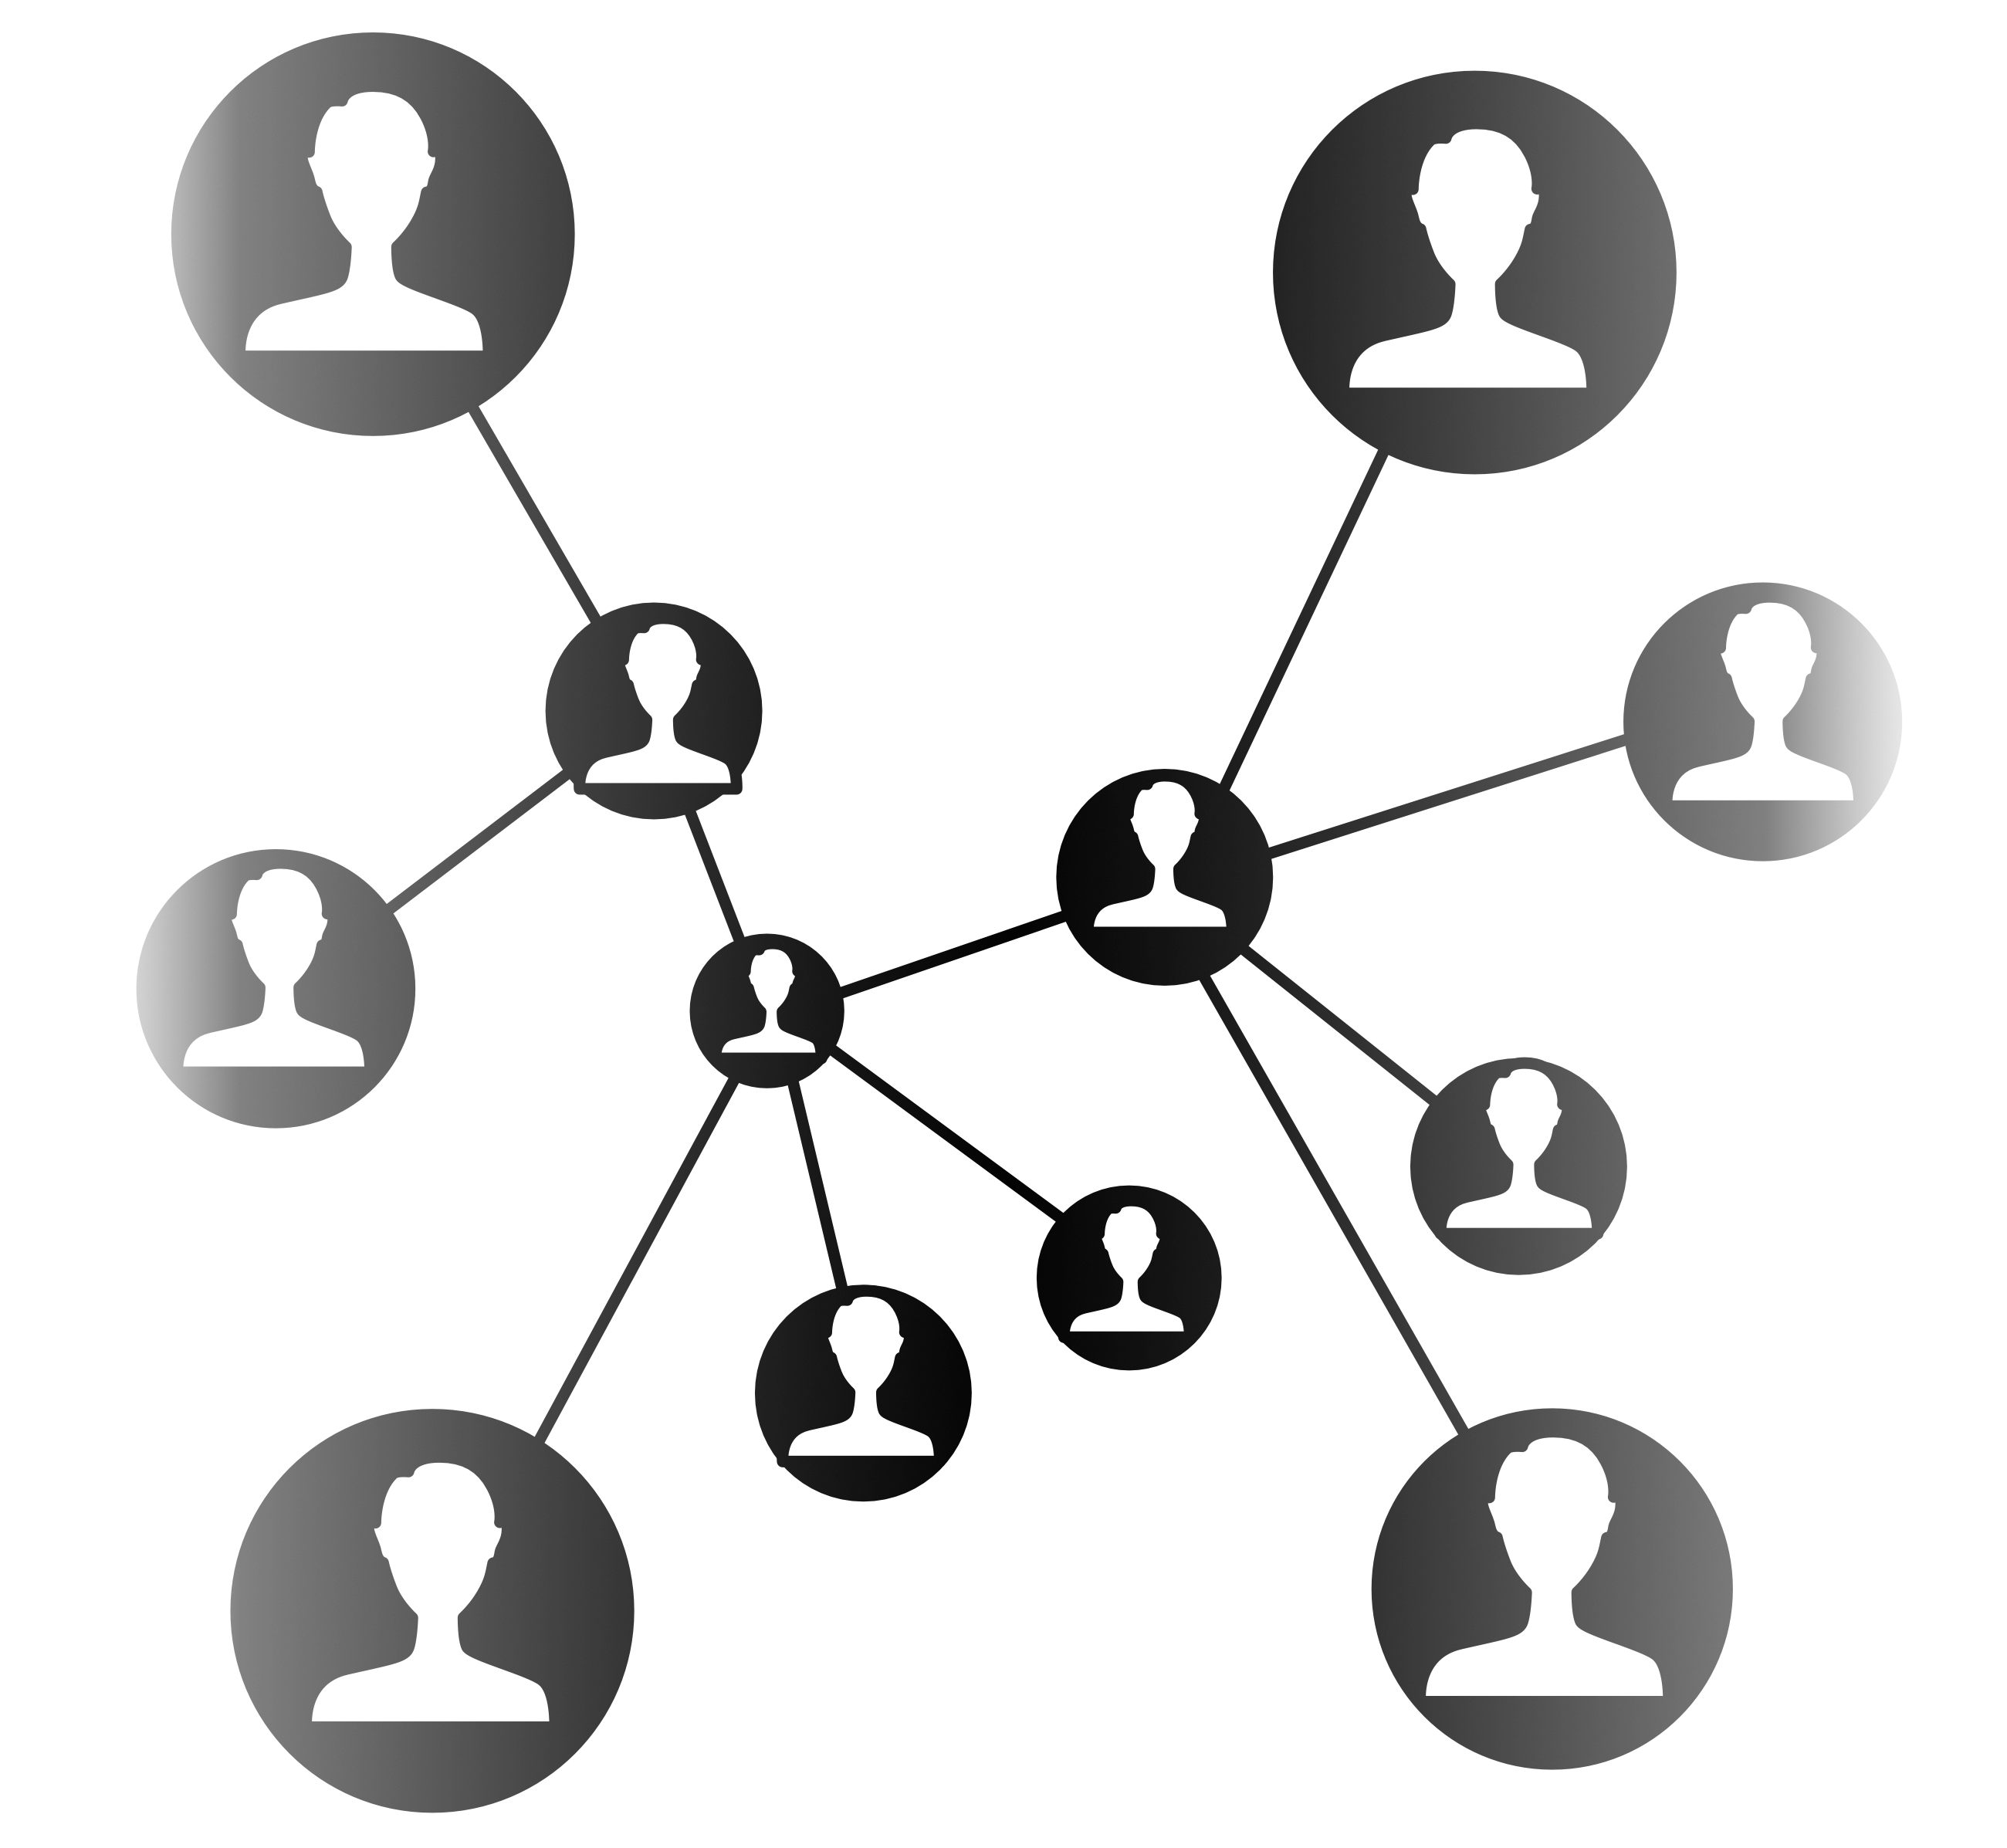
\includegraphics[width=\textwidth]{figures/networkTransparency.png}
    }
  \end{figure}

\end{column}

\begin{column}[T]{0.25\textwidth}
\centering
\vspace{5mm}

\visible<2->{
  \small{Complexity}
  \vspace{13mm}
}

\small{Tasks}

\visible<3->{
  \vspace{11mm}
  \small{Decomposition}
}

\end{column}
\end{columns}
\end{frame}


\begin{frame}[standout]
    What will be the future of work?
\end{frame}

\begin{frame}{What will be the future of work?}
    How will \alert{technology} affect the complexity of the work that on--demand workers do?

    What are the \alert{limits} of complexity in on--demand work?

    How can we \alert{reach} those limits?
\end{frame}


\begin{frame}{Thesis}
    These questions have all been asked before.

    History can help us answer them today.

    We'll reach into the history of \alert{piecework}
    --- of human computers, match stick makers, and metalworkers ---
    and show how the \alert{history} of their work can
    inform answers to questions about the \alert{future} of digital work.
\end{frame}

\againframe<4->{returnable}

\notinsubfile{
  \subfile{timeline.tex} % this takes a while to compile...
}


\begin{frame}{Introduction}
  We hope to provide:
      \begin{itemize}
        \item A useful ontological lens for making sense of on--demand work as a resurgence of \alert{piecework}.
        \item A method for making sense of contemporary phenomena through \alert{historical analysis}.
      \end{itemize}
\end{frame}


\begin{frame}{Comparative Historical Analysis}
\begin{itemize}
  \item Historical analysis isn't new
  \begin{itemize}
    \item In general\\
    \scriptsize{
      \textcite{rosenberg1994exploring,rosenberg1982inside}
    }
    \item In HCI\\
    \scriptsize{
      \textcite{Wyche2006,bodker1993historical}
    }
  \end{itemize}
  \item Still, it's an underutilized method
  \begin{itemize}
    \item Provide some basic framing for \emph{ostensibly} new phenomena
    \item \emph{Explicate} our theoretical grounding
    \item Flesh out \emph{differences} and their implications
  \end{itemize}
\end{itemize}
\end{frame}



\onlyinsubfile{
  \printbibliography{}
}

\end{document}